\documentclass{beamer}

\newcommand{\course}{CS 2340 Objects and Design}
\newcommand{\lesson}{Object-Oriented Design}
\newcommand{\code}{http://www.cc.gatech.edu/~simpkins/teaching/gatech/cs2340/code}

\author[Chris Simpkins] 
{Christopher Simpkins \\\texttt{chris.simpkins@gatech.edu}}
\institute[Georgia Tech] % (optional, but mostly needed)

\date[CS 1331]{}

\subject{\lesson}


% If you have a file called "university-logo-filename.xxx", where xxx
% is a graphic format that can be processed by latex or pdflatex,
% resp., then you can add a logo as follows:

% \pgfdeclareimage[width=0.6in]{coc-logo}{cc_2012_logo}
% \logo{\pgfuseimage{coc-logo}}

\mode<presentation>
{
  \usetheme{Berlin}
  \useoutertheme{infolines}

  % or ...

 \setbeamercovered{transparent}
  % or whatever (possibly just delete it)
}

\usepackage{hyperref}
\usepackage{fancybox}
\usepackage{listings}
\usepackage[abbr]{harvard}

\usepackage[english]{babel}
% or whatever

\usepackage[latin1]{inputenc}
% or whatever

\usepackage{times}
\usepackage[T1]{fontenc}
% Or whatever. Note that the encoding and the font should match. If T1
% does not look nice, try deleting the line with the fontenc.


\usepackage{listings}
 
% "define" Scala
\lstdefinelanguage{scala}{
  morekeywords={abstract,case,catch,class,def,%
    do,else,extends,false,final,finally,%
    for,if,implicit,import,match,mixin,%
    new,null,object,override,package,%
    private,protected,requires,return,sealed,%
    super,this,throw,trait,true,try,%
    type,val,var,while,with,yield},
  otherkeywords={=>,<-,<\%,<:,>:,\#,@},
  sensitive=true,
  morecomment=[l]{//},
  morecomment=[n]{/*}{*/},
  morestring=[b]",
  morestring=[b]',
  morestring=[b]""",
}

\usepackage{color}
\definecolor{dkgreen}{rgb}{0,0.6,0}
\definecolor{gray}{rgb}{0.5,0.5,0.5}
\definecolor{mauve}{rgb}{0.58,0,0.82}
 
% Default settings for code listings
\lstset{frame=tb,
  language=scala,
  aboveskip=2mm,
  belowskip=2mm,
  showstringspaces=false,
  columns=flexible,
  basicstyle={\scriptsize\ttfamily},
  numbers=none,
  numberstyle=\tiny\color{gray},
  keywordstyle=\color{blue},
  commentstyle=\color{dkgreen},
  stringstyle=\color{mauve},
  frame=single,
  breaklines=true,
  breakatwhitespace=true,
  keepspaces=true
  %tabsize=3
}


\title[\course] % (optional, use only with long
                                      % paper titles)
{\lesson}

\subtitle{}
%% {Include Only If Paper Has a Subtitle}

\newcommand{\link}[2]{\href{#1}{\textcolor{blue}{\underline{#2}}}}


% \beamerdefaultoverlayspecification{<+->}


\begin{document}

\begin{frame}
  \titlepage
\end{frame}



%------------------------------------------------------------------------
\begin{frame}[fragile]{Object-Oriented Design}


Engineering design
\begin{quote}
A systematic, intelligent process in which designers generate, evaluate and specify designs for devices, systems, or processes whose form(s) and function(s) acheive clients' objectives and users' needs while satisfying a specified set of constraints. -- Dym and Little, quoted in Carlos Otero, Software Engineering Design
\end{quote}
Object-oriented design:
\begin{itemize}
\item identifying problem domain objects and representing them with classes (classes),
\item factoring classes so they have the right granularity (responsibilities),
\begin{itemize}
\item typically means defining class and interface hierarchies
\end{itemize}
\item defining relationships between the classes (collaborations).
\end{itemize}
\end{frame}
%------------------------------------------------------------------------

%------------------------------------------------------------------------
\begin{frame}[fragile]{Object-Oriented Design Principles}

\begin{itemize}
\item {\bf S}ingle Responsibility Principle
\item {\bf O}pen Closed Principle
\item {\bf L}iskov Substitution Principle
\item {\bf I}nterface Segregation Principle
\item {\bf D}ependency Inversion Principle
\end{itemize}

\end{frame}
%------------------------------------------------------------------------

%------------------------------------------------------------------------
\begin{frame}[fragile]{Single Responsibility Principle (SRP)}

\begin{quote}
A class should have only one reason to change.
\end{quote}

\begin{itemize}
\item A responsiblity is an axis of change.
\item Classes with multiple responsiblities will couple the responsibilities, making changes to one responsilbity more difficult due to the risk of breaking the other responsibilities handled by the class.
\end{itemize}


\end{frame}
%------------------------------------------------------------------------

%------------------------------------------------------------------------
\begin{frame}[fragile]{SRP Example - Too Many Responsibilities}

\vspace{-.1in}
\begin{lstlisting}[language=Java]
public class GreetingFrame extends JFrame implements ActionListener {
    private JLabel greetingLabel;

    public GreetingFrame() {
        ...
        JButton button = new JButton("Greet!");
        button.addActionListener(this);
        ...
    }
    public void actionPerformed(ActionEvent e) {
        Greeter greeter = new Greeter("bob");
        String greeting = greeter.greet();
        greetingLabel.setText(greeting);
    }
}
\end{lstlisting}
\vspace{-.1in}
\begin{itemize}
\item If we add other buttons or menu items to the GUI, we have to modify the {\tt actionPerformed} method to handle an additional event source.
\item If we chnage the behavior of the a button, we have to modify the {\tt actoinPerformed} method.
\end{itemize}


\end{frame}
%------------------------------------------------------------------------

%------------------------------------------------------------------------
\begin{frame}[fragile]{SRP Example - Single-Responsibility Classes}
\vspace{-.1in}
\begin{lstlisting}[language=Java]
private class GreetButtonListener implements ActionListener {
  private JLabel greetingLabel;
  
  public GreetButtonListener(JLabel greetingLabel) {
    this.greetingLabel = greetingLabel;
  }
  public void actionPerformed(ActionEvent e) {
    ...
  }
}
public class GreetingFrame extends JFrame {
  ...
  public GreetingFrame() {
    ...
    button.addActionListener(new GreetButtonListener(greetingLabel)); 
    ...
  }
}
\end{lstlisting}
\vspace{-.1in}
\begin{itemize}
\item Additions to the UI require changes only to {\tt GreetingFrame}.
\item Changes to greet button behavior require changes only to {\tt GreetButtonListener}.
\end{itemize}


\end{frame}
%------------------------------------------------------------------------


%------------------------------------------------------------------------
\begin{frame}[fragile]{Open--Closed Principle (OCP)}

\begin{quote}
Software Entities (classes, modules, functions) should be open for extension, but closed for modification.
\end{quote}

\begin{itemize}
\item Open for extension means the module should be extendable with new behavior.
\item Closed for modification means the module shouldn't need to be touched in order to add the extension.
\end{itemize}
Object-oriented polymorphism makes this possible, namely, to write new code that works with old code without having to touch the old code.


\end{frame}
%------------------------------------------------------------------------

%------------------------------------------------------------------------
\begin{frame}[fragile]{OCP Example}

\begin{lstlisting}[language=Java]
public abstract class Sql {
  public Sql(String table, Column[] columns)
  public abstract String generate();
}
public class CreateSql extends Sql {
  public CreateSql(String table, Column[] columns)
  @Override public String generate()
}
public class SelectSql extends Sql {
  public SelectSql(String table, Column[] columns)
  @Override public String generate()
}
...
\end{lstlisting}

These classes are open for extension and closed for modification.
\begin{itemize}
\item Extend with new functionality by adding a new subclass of {\tt Sql}.
\item Existing classes need not be touched.
\end{itemize}

\end{frame}
%------------------------------------------------------------------------

%------------------------------------------------------------------------
\begin{frame}[fragile]{Liskov Substitution Principle (LSP)}
\vspace{-.05in}
\begin{quote}
Subtypes must be substitutable for their supertypes.
\end{quote}
\vspace{-.075in}
A suprising counter-example:
\vspace{-.05in}
\begin{lstlisting}[language=Java]
public class Rectangle {
  public void setWidth(double w) { ... }
  public void setHeight(double h) { ... }
}
public class Square extends Rectangle {
  public void setWidth(double w) {
    super.setWidth(w);
    super.setHeight(w);
  }
  public void setHeight(double h) {
    super.setWidth(h);
    super.setHeight(h);
  }
}
\end{lstlisting}
\vspace{-.1in}
\begin{itemize}
\item We know from math class that a square ``is a'' rectangle. 
\item The overridden {\tt setWidth} and {\tt setHeight} methods in {\tt Square} enforce the class invariant of {\tt Square}, namely, that {\tt width == height}.
\end{itemize}


\end{frame}
%------------------------------------------------------------------------

%------------------------------------------------------------------------
\begin{frame}[fragile]{LSP Violation}


Consider this client of {\tt Rectangle}:
\begin{lstlisting}[language=Java]
public void g(Rectangle r) {
  r.setWidth(5);
  r.setHeight(4);
  assert(r.area() == 20);
}
\end{lstlisting}

\begin{itemize}
\item Client assumed width and height were independent.
\end{itemize}
The Object-oriented {\tt is-a} relationship is about behavior.

\end{frame}
%------------------------------------------------------------------------

%------------------------------------------------------------------------
\begin{frame}[fragile]{Conforming to LSP: Design by Contract}


Author of a class specifies the behavior of each method in terms of preconditions and postconditions.  Subclasses must follow two rules:
\begin{itemize}
\item Preconditions of overriden methods must be equal to or weaker than those of the superclass (enforces or assumes no more than the constraints of the superclass method).
\item Postconditins of overriden methods must be equal to or greater than those of the superclass (enforces all of the constraints of the superclas method and possibly more).
\end{itemize}

\begin{quote}
Require no more, promise no less.
\end{quote}

In the Rectangle-Square case the postcondition of {\tt Rectangle}'s {\tt setWidth} method:
\begin{lstlisting}
assert((rectangle.w == w) && (rectangle.height == old.height))
\end{lstlisting}
tells us that a {\tt Square} doesn't satisfy the object-oriented {\it is-a} relationship to {\tt Rectangle}.

\end{frame}
%------------------------------------------------------------------------


%------------------------------------------------------------------------
\begin{frame}[fragile]{Dependency Inversion Principle (DIP)\footnote{A.K.A. Dependency Injection}}
\vspace{-.05in}
\begin{quote}
a. High-level modules should not depend on low-level modules.  Both should depend on abstractions.\\
b. Abstractions should not depend on details.  Details should depend on abstractions.
\end{quote}
\vspace{-.1in}
A counter-example:
\vspace{-.05in}
\begin{lstlisting}[language=Java]
public void regulate(double minTemp, double maxTemp) {
  for (;;) {
    while (in(THERMOMETER) > minTemp)
      Thread.sleep(1000);
    out(FURNACE, ENGAGE);

    while (inTHERMOMETER) < maxTemp)
      Thread.sleep(1000);
   out(FURNACE, DISENGAGE);
  }
}
\end{lstlisting}
\vspace{-.125in}
\begin{itemize}
\item The {\tt regulate} method depends on a particular thermometer and furnace implementation.
\item The regulate algorithm is cluttered with low-level details of the thermometer and furnace operations.
\end{itemize}


\end{frame}
%------------------------------------------------------------------------

%------------------------------------------------------------------------
\begin{frame}[fragile]{DIP Example}
\vspace{-.1in}
\begin{columns}[c]

\begin{column}{2.25in}
\begin{center}
\includegraphics[width=2.2in]{thermostat-dip-uml.png}
\end{center}
\end{column}

\begin{column}{2.75in}
\begin{lstlisting}[language=Java]
public void regulate(double minTemp,
                     double maxTemp){
  for (;;) {
    while (thermometer.read() > minTemp)
      Thread.sleep(1000);
    heater.engage();

    while (thermometer.read() < maxTemp)
      Thread.sleep(1000);
    heater.disengage();
  }
}
\end{lstlisting}
\end{column}
\end{columns}
\vspace{-.1in}
\begin{itemize}
\item {\tt Thermostat} depends on interfaces {\tt Thermometer} and {\tt Heater}
\item Concrete heaters and thermometers also depend on {\tt Thermometer} and {\tt Heater}
\item Low-level detail is removed form {\tt regulate} method
\item Can be extended with different concrete implementations of {\tt Thermometer} and {\tt Heater} while maintaining OCP
\end{itemize}


\end{frame}
%------------------------------------------------------------------------


%------------------------------------------------------------------------
\begin{frame}[fragile]{Interface Segregation Principle (ISP)}
\vspace{-.05in}
\begin{quote}
Clients should not be forced to depend on methods they don't use.
\end{quote}
Break up fat interfaces into a set of smaller interfaces.  Each client depends on the small interface it needs, and none of the others.
\vspace{-.05in}
\begin{center}
\includegraphics[width=2.2in]{fat-atm-ui.png}
\end{center}
\vspace{-.2in}
\begin{itemize}
\item Additional UI methods in {\tt UI} require recompilation of all the transaction classes, even the ones that don't use the new methods.
\end{itemize}


\end{frame}
%------------------------------------------------------------------------

%------------------------------------------------------------------------
\begin{frame}[fragile]{ISP Example}

\vspace{-.1in}
Segregated UI interfaces:
\vspace{-.1in}
\begin{center}
\includegraphics[width=3in]{factored-atm-ui.png}
\end{center}
\vspace{-.3in}
\begin{itemize}
\item Each transaction gets its own UI interface.
\item Adding transactions doesn't require touching or recompiling other transactions or UIs.
\end{itemize}


\end{frame}
%------------------------------------------------------------------------

%------------------------------------------------------------------------
\begin{frame}[fragile]{Design Patterns}


\begin{columns}[c]

\begin{column}{2in}
\begin{center}
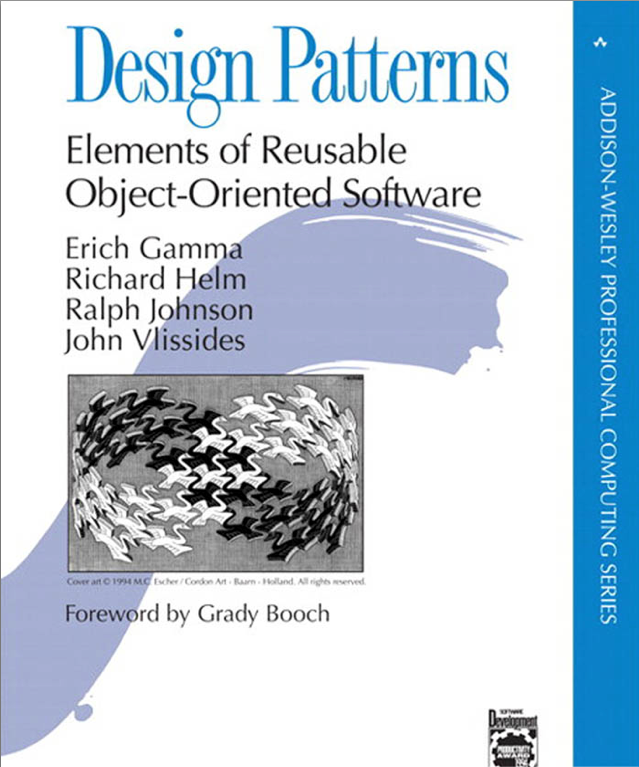
\includegraphics[width=1.9in]{design-patterns-book.png}
\end{center}
\end{column}

\begin{column}{3in}
A recurring object-oriented design.
\begin{itemize}
\item Make proven techniques more accessible to developers of new systems -- don't have to study other systems.
\item Helps in choosing designs that make the system more reusable.
\item Facilitate documenentation and communication with other developers.
\end{itemize}
Design pattern catalog: descriptions of communicating objects and classes that are customized to solve a general design problem in a particular context.

\end{column}

\end{columns}

\end{frame}
%------------------------------------------------------------------------

%------------------------------------------------------------------------
\begin{frame}[fragile]{Common Design Patterns}

\begin{itemize}
\item {\bf Abstract Factory} Provide an interface for creating families of related or dependent objects without specifying their concrete classes. (GoF, 87)
\item {\bf Factory Method} Define an interface for creating an object, but let subclasses decide which class to instantiate. Factory Method lets a class defer instantiation to subclasses. (GoF, 107)
\item {\bf Adapter} Convert the interface of a class into another interface clients expect. Adapter lets classes work together that couldn't otherwise because of incompat ible interfaces. (GoF, 139)
\item {\bf Composite} Compose objects into tree structures to represent part-whole hierarchies. Composite lets clients treat individual objects and compositions of objects uniformly. (GoF, 163)
\end{itemize}


\end{frame}
%------------------------------------------------------------------------

%------------------------------------------------------------------------
\begin{frame}[fragile]{Common Design Patterns}

\begin{itemize}
\item {\bf Decorator} Attach additional responsibilities to an object dynamically. Decorators provide a flexible alternative to subclassing for extending functionality. (GoF, 175)
\item {\bf Observer} Define a one-to-many dependency between objects so that when one object changes state, all its dependents are notified and updated automatically. (GoF, 293)
\item {\bf Strategy} Define a family of algorithms, encapsulate each one, and make them interchangeable. Strategy lets the algorithm vary independently from clients that use it. (GoF, 315)
\item {\bf Template Method} Define the skeleton of an algorithm in an operation, deferring some steps to subclasses. Template Method lets subclasses redefine certain steps of an algorithm without changing the algorithm's structure. (GoF, 325)
\end{itemize}


\end{frame}
%------------------------------------------------------------------------


% %------------------------------------------------------------------------
% \begin{frame}[fragile]{}


% \begin{lstlisting}[language=Java]

% \end{lstlisting}

% \begin{itemize}
% \item
% \end{itemize}


% \end{frame}
% %------------------------------------------------------------------------


\end{document}
